\clearpage
\section{Complete estimates and sensitivity results}
\label{app:results}

Tables~\ref{tab:global-estimates}--\ref{tab:run-stability} report the global and legacy
within-metric results with standard errors, intervals, randomization $p$-values, and
multiplicity adjustments. Negative target-loss contrasts favor GPT-5.6 Sol; for VDR the
loss is $|\VDR-1|$, and for CSR it is $1-\CSR$. The five-metric global family supports
one corrected conclusion: TVD improves.

\begin{table}[!htbp]
\centering
\caption{Global model estimates. Standard errors and BCa intervals resample countries in 20,000 draws.}
\label{tab:global-estimates}
\small
\begin{tabular}{llrrr}
\toprule
\rowcolor{tablehead} Model & Metric & Estimate & SE & 95\% BCa CI \\
\midrule
GPT-5.5 & W1 & 0.1284 & 0.0052 & [0.1187,0.1392] \\
GPT-5.5 & TVD & 0.3124 & 0.0092 & [0.2953,0.3318] \\
GPT-5.5 & CRG & 1.0469 & 0.0449 & [0.9576,1.1193] \\
GPT-5.5 & VDR & 0.5873 & 0.0358 & [0.5183,0.6579] \\
GPT-5.5 & CSR & 0.3211 & 0.0767 & [0.1560,0.4470] \\
GPT-5.6 Sol & W1 & 0.1265 & 0.0050 & [0.1171,0.1369] \\
GPT-5.6 Sol & TVD & 0.3043 & 0.0088 & [0.2883,0.3230] \\
GPT-5.6 Sol & CRG & 1.0447 & 0.0448 & [0.9533,1.1160] \\
GPT-5.6 Sol & VDR & 0.6093 & 0.0359 & [0.5383,0.6779] \\
GPT-5.6 Sol & CSR & 0.2878 & 0.0787 & [0.1122,0.4157] \\
\bottomrule
\end{tabular}
\end{table}
\begin{table}[!htbp]
\centering
\caption{Global target-loss contrasts. Negative estimates favor GPT-5.6 Sol.}
\label{tab:global-contrasts}
\small
\begin{tabular}{lrrrrr}
\toprule
\rowcolor{tablehead} Metric & $\Delta$ loss & SE & 95\% BCa CI & $p_{\rm perm}$ & Holm $p$ \\
\midrule
W1 & -0.0020 & 0.0011 & [-0.0040,0.0003] & 0.07975 & 0.31900 \\
\rowcolor{improvebg}
TVD & -0.0080 & 0.0014 & [-0.0107,-0.0050] & 0.00005 & 0.00025 \\
CRG & -0.0022 & 0.0117 & [-0.0243,0.0215] & 0.84455 & 0.84455 \\
VDR & -0.0220 & 0.0135 & [-0.0506,0.0025] & 0.09580 & 0.31900 \\
CSR & 0.0333 & 0.0232 & [-0.0082,0.0834] & 0.15290 & 0.31900 \\
\bottomrule
\end{tabular}
\end{table}
\FloatBarrier
\begin{table}[!htbp]
\centering
\small
\setlength{\tabcolsep}{1.8pt}
\caption{Domain W1 estimates and paired contrasts. Model cells report estimate (country-bootstrap SE); $\Delta$ is GPT-5.6 Sol minus GPT-5.5 and negative values favor GPT-5.6 Sol.}\label{tab:domain-w1}
\begin{tabular}{@{}lrrrrrr@{}}
\toprule
\rowcolor{tablehead} Domain & 5.5 (SE) & 5.6 (SE) & $\Delta$ (SE) & 95\% BCa CI & $p_{\rm perm}$ & Holm $p$ \\
\midrule
Agency & .1385 (.0090) & .1352 (.0085) & -.0033 (.0021) & [-.0073,.0007] & .11395 & .34185 \\
Trust & .1043 (.0103) & .1075 (.0103) & .0032 (.0037) & [-.0035,.0111] & .39615 & .79230 \\
\rowcolor{improvebg}
Distribution & .1833 (.0112) & .1746 (.0109) & -.0087 (.0030) & [-.0141,-.0021] & .00545 & .02725 \\
\rowcolor{improvebg}
Responsibility & .1359 (.0072) & .1276 (.0068) & -.0082 (.0025) & [-.0127,-.0028] & .00135 & .00810 \\
Immigration & .0969 (.0061) & .1018 (.0063) & .0049 (.0023) & [.0003,.0091] & .03240 & .12960 \\
Science & .1117 (.0072) & .1121 (.0073) & .0004 (.0016) & [-.0028,.0034] & .80615 & .80615 \\
\bottomrule
\end{tabular}
\end{table}
\begin{table}[!htbp]
\centering
\small
\setlength{\tabcolsep}{1.8pt}
\caption{Domain TVD estimates and paired contrasts. Model cells report estimate (country-bootstrap SE); $\Delta$ is GPT-5.6 Sol minus GPT-5.5 and negative values favor GPT-5.6 Sol.}\label{tab:domain-tvd}
\begin{tabular}{@{}lrrrrrr@{}}
\toprule
\rowcolor{tablehead} Domain & 5.5 (SE) & 5.6 (SE) & $\Delta$ (SE) & 95\% BCa CI & $p_{\rm perm}$ & Holm $p$ \\
\midrule
Agency & .4055 (.0172) & .4005 (.0166) & -.0050 (.0023) & [-.0095,-.0003] & .03605 & .10815 \\
Trust & .1043 (.0103) & .1075 (.0103) & .0032 (.0037) & [-.0035,.0111] & .40180 & .40180 \\
\rowcolor{improvebg}
Distribution & .4164 (.0158) & .3898 (.0141) & -.0266 (.0042) & [-.0348,-.0184] & .00005 & .00030 \\
\rowcolor{improvebg}
Responsibility & .3940 (.0139) & .3733 (.0128) & -.0207 (.0032) & [-.0268,-.0144] & .00005 & .00030 \\
Immigration & .2208 (.0093) & .2287 (.0098) & .0078 (.0037) & [.0005,.0149] & .03885 & .10815 \\
\rowcolor{improvebg}
Science & .3332 (.0154) & .3262 (.0156) & -.0070 (.0024) & [-.0118,-.0023] & .00660 & .02640 \\
\bottomrule
\end{tabular}
\end{table}
\FloatBarrier
\begin{table}[!htbp]
\centering
\caption{Q121 label-conflict sensitivity. The relabeling scenarios move the stated fraction of each model's category-1 mass to category 2; they bound scoring effects and do not recreate model generation.}
\label{tab:q121-sensitivity}
\small
\begin{tabular}{llrrr}
\toprule
\rowcolor{tablehead} Scenario & Metric & $\Delta$ & 95\% BCa CI & Holm $p$ \\
\midrule
as collected & W1 & 0.0049 & [0.0003,0.0091] & 0.0723 \\
as collected & TVD & 0.0078 & [0.0006,0.0149] & 0.0723 \\
50\% shift & W1 & 0.0032 & [-0.0015,0.0075] & 0.3344 \\
50\% shift & TVD & 0.0042 & [-0.0024,0.0108] & 0.3344 \\
100\% shift & W1 & 0.0037 & [-0.0006,0.0077] & 0.0894 \\
100\% shift & TVD & 0.0076 & [0.0002,0.0147] & 0.0894 \\
\bottomrule
\end{tabular}
\end{table}
\begin{table}[!htbp]
\centering
\caption{Conditional uncertainty decomposition. These centered sensitivity intervals hold countries fixed; they complement, not replace, Table~\ref{tab:global-contrasts}.}
\label{tab:conditional-uncertainty}
\small
\begin{tabular}{llrr}
\toprule
\rowcolor{tablehead} Source & Metric & Conditional SE & Centered 95\% interval \\
\midrule
human cells & W1 & 0.0006 & [-0.0031,-0.0009] \\
human cells & TVD & 0.0007 & [-0.0095,-0.0066] \\
human cells & CRG & 0.0044 & [-0.0109,0.0066] \\
human cells & VDR & 0.0004 & [-0.0229,-0.0212] \\
human cells & CSR & 0.0130 & [0.0078,0.0583] \\
five generations & W1 & 0.0005 & [-0.0030,-0.0009] \\
five generations & TVD & 0.0007 & [-0.0094,-0.0067] \\
five generations & CRG & 0.0061 & [-0.0140,0.0097] \\
five generations & VDR & 0.0049 & [-0.0317,-0.0123] \\
five generations & CSR & 0.0102 & [0.0130,0.0529] \\
\bottomrule
\end{tabular}
\end{table}
\FloatBarrier
\begin{table}[!htbp]
\centering
\small
\setlength{\tabcolsep}{2.0pt}
\caption{Signed expected-score bias by model and domain. Positive values indicate a higher expected directed response than the human derivative; these signs are descriptive, not normative.}\label{tab:signed-bias}
\begin{tabular}{@{}llrrrrr@{}}
\toprule
\rowcolor{tablehead} Model & Domain & Bias & SE & 95\% BCa CI & $p_{\rm perm}$ & Holm $p$ \\
\midrule
GPT-5.5 & Agency & -.1067 & .0122 & [-.1311,-.0833] & .00005 & .00030 \\
GPT-5.5 & Trust & .0363 & .0158 & [.0045,.0667] & .02705 & .05410 \\
GPT-5.5 & Distribution & .1000 & .0201 & [.0596,.1390] & .00010 & .00040 \\
GPT-5.5 & Responsibility & -.0019 & .0146 & [-.0324,.0253] & .90110 & .90110 \\
GPT-5.5 & Immigration & .0290 & .0113 & [.0058,.0502] & .01290 & .03870 \\
GPT-5.5 & Science & -.0775 & .0102 & [-.0978,-.0576] & .00005 & .00030 \\
GPT-5.6 Sol & Agency & -.1047 & .0118 & [-.1280,-.0817] & .00005 & .00030 \\
GPT-5.6 Sol & Trust & .0298 & .0163 & [-.0035,.0603] & .07600 & .15200 \\
GPT-5.6 Sol & Distribution & .0880 & .0202 & [.0473,.1265] & .00010 & .00040 \\
GPT-5.6 Sol & Responsibility & .0088 & .0141 & [-.0202,.0351] & .53600 & .53600 \\
GPT-5.6 Sol & Immigration & .0294 & .0121 & [.0047,.0519] & .01760 & .05280 \\
GPT-5.6 Sol & Science & -.0803 & .0104 & [-.1010,-.0600] & .00005 & .00030 \\
\bottomrule
\end{tabular}
\end{table}
\begin{table}[!htbp]
\centering
\caption{Bootstrap-draw convergence. Values are the maximum absolute movement, across the two models, of either percentile-interval endpoint between 10,000 and 20,000 country resamples.}\label{tab:bootstrap-convergence}
\small
\begin{tabular}{lr}
\toprule
\rowcolor{tablehead} Metric & Maximum endpoint movement \\
\midrule
W1 & 0.00026 \\
TVD & 0.00034 \\
CRG & 0.00225 \\
VDR & 0.00081 \\
CSR & 0.00227 \\
\bottomrule
\end{tabular}
\end{table}
\begin{table}[!htbp]
\centering
\caption{Within-cell run instability across five generations. Values summarize the SD across generations within each country--question cell.}
\label{tab:run-stability}
\small
\begin{tabular}{llrrr}
\toprule
\rowcolor{tablehead} Model & Scope & Cells & Mean SD W1 & Mean SD TVD \\
\midrule
GPT-5.5 & all anchors & 384 & 0.0148 & 0.0207 \\
GPT-5.6 Sol & all anchors & 384 & 0.0161 & 0.0211 \\
\bottomrule
\end{tabular}
\end{table}
\FloatBarrier


Table~\ref{tab:joint-items} gives the stricter joint item family used for current claims.
Q108 improves under W1 and TVD, and Q106 improves under TVD; Q106 W1 and Q159 TVD
narrowly miss the 5\% familywise threshold. Tables~\ref{tab:composition}--\ref{tab:cell-quartiles}
then report composition, creative-destruction margins, and influence analyses.

\subsection{Joint item-level inference}
\begin{longtable}{llrrrr}
\caption{All 12 item-level contrasts in one max-$T$ family. Negative values favor GPT-5.6. SEs use countries; intervals are simultaneous 95\% bootstrap intervals.}\label{tab:joint-items}\\
\toprule
\rowcolor{tablehead} Metric & Item & $\Delta$ & SE & Simultaneous 95\% CI & max-$T$ $p$ \\
\midrule\endfirsthead\toprule
\rowcolor{tablehead} Metric & Item & $\Delta$ & SE & Simultaneous 95\% CI & max-$T$ $p$ \\\midrule\endhead
W1 & Agency (Q48) & -0.0033 & 0.0021 & [-0.0094,0.0028] & 0.65550 \\
W1 & Trust (Q57) & 0.0032 & 0.0038 & [-0.0077,0.0142] & 0.98840 \\
W1 & Distribution (Q106) & -0.0087 & 0.0030 & [-0.0176,0.0002] & 0.05915 \\
\rowcolor{improvebg}
W1 & Responsibility (Q108) & -0.0082 & 0.0025 & [-0.0156,-0.0009] & 0.01735 \\
W1 & Immigration (Q121) & 0.0049 & 0.0023 & [-0.0018,0.0116] & 0.28060 \\
W1 & Science (Q159) & 0.0004 & 0.0016 & [-0.0042,0.0050] & 1.00000 \\
TVD & Agency (Q48) & -0.0050 & 0.0024 & [-0.0119,0.0019] & 0.28545 \\
TVD & Trust (Q57) & 0.0032 & 0.0038 & [-0.0077,0.0142] & 0.98840 \\
\rowcolor{improvebg}
TVD & Distribution (Q106) & -0.0266 & 0.0042 & [-0.0389,-0.0143] & 0.00005 \\
\rowcolor{improvebg}
TVD & Responsibility (Q108) & -0.0207 & 0.0032 & [-0.0301,-0.0113] & 0.00005 \\
TVD & Immigration (Q121) & 0.0078 & 0.0037 & [-0.0030,0.0186] & 0.29595 \\
TVD & Science (Q159) & -0.0070 & 0.0024 & [-0.0141,0.0001] & 0.05580 \\
\bottomrule\end{longtable}
\clearpage
\subsection{Finite-five-generation composition diagnostic}
\begin{table}[!htbp]\centering\small
\caption{Squared probability error decomposed into the residual after averaging the observed five runs and their generation-varying component. This finite-pool identity is not an asymptotic bias estimate. Country-bootstrap SEs and 95\% BCa intervals are reported.}\label{tab:composition}
\begin{tabular}{llrrr}\toprule
\rowcolor{tablehead} Comparison & Component & Estimate & SE & 95\% BCa CI \\\midrule
5.5 & single-generation error & 0.11121 & 0.00807 & [0.09768,0.13003] \\
5.5 & five-run residual & 0.10990 & 0.00806 & [0.09638,0.12873] \\
5.5 & generation-varying & 0.00131 & 0.00006 & [0.00121,0.00144] \\
5.5 & share removed by mean & 1.180\% & 0.090\% & [1.018,1.371]\% \\
5.6 & single-generation error & 0.10494 & 0.00763 & [0.09209,0.12284] \\
5.6 & five-run residual & 0.10357 & 0.00761 & [0.09078,0.12140] \\
5.6 & generation-varying & 0.00138 & 0.00006 & [0.00126,0.00151] \\
5.6 & share removed by mean & 1.313\% & 0.092\% & [1.147,1.509]\% \\
5.6 $-$ 5.5 & single-generation error & -0.00627 & 0.00097 & [-0.00826,-0.00447] \\
5.6 $-$ 5.5 & five-run residual & -0.00633 & 0.00097 & [-0.00834,-0.00452] \\
5.6 $-$ 5.5 & generation-varying & 0.00007 & 0.00006 & [-0.00004,0.00018] \\
\bottomrule\end{tabular}\end{table}
\subsection{Creative-destruction margins and weight sensitivity}
\begin{table}[!htbp]\centering\small
\caption{Exploratory theory-indexed margins, using mean squared TVD. Negative contrasts favor GPT-5.6. Holm correction spans three margins.}\label{tab:economic-margins}
\begin{tabular}{lrrrrr}\toprule
\rowcolor{tablehead} Margin & GPT-5.5 & GPT-5.6 & $\Delta$ (SE) & 95\% BCa CI & Holm $p$ \\\midrule
\rowcolor{improvebg}
Opportunity/participation & 0.15467 & 0.15000 & -0.00467 (0.00144) & [-0.00753,-0.00190] & 0.00350 \\
\rowcolor{improvebg}
Distribution/adjustment & 0.17839 & 0.15706 & -0.02133 (0.00260) & [-0.02638,-0.01614] & 0.00015 \\
Coordination/legitimacy & 0.03588 & 0.03826 & 0.00238 (0.00127) & [-0.00005,0.00492] & 0.06710 \\
\bottomrule\end{tabular}\end{table}
\begin{table}[!htbp]\centering\small
\caption{Selected nonnegative weighting scenarios. Weights sum to one. Intervals use the paired country bootstrap.}\label{tab:economic-scenarios}
\begin{tabular}{lrrrr}\toprule
\rowcolor{tablehead} Scenario & $\Delta$ weighted loss & SE & 95\% CI & $P(\Delta<0)$ \\\midrule
\rowcolor{improvebg}
Equal weights & -0.0079 & 0.0010 & [-0.0099,-0.0058] & 1.000 \\
\rowcolor{improvebg}
Opportunity only & -0.0047 & 0.0014 & [-0.0075,-0.0019] & 0.999 \\
\rowcolor{improvebg}
Distribution only & -0.0213 & 0.0026 & [-0.0264,-0.0162] & 1.000 \\
Coordination only & 0.0024 & 0.0013 & [-0.0001,0.0049] & 0.030 \\
\bottomrule\end{tabular}\end{table}
Across the full 0.02 weight grid (1326 points), 88.76\% of 95\% intervals favor GPT-5.6, 11.24\% are uncertain, and none favor GPT-5.5. This is a sensitivity analysis over a declared index, not an observed welfare estimate.
\subsection{Influence of regions and human-cell size}
\begin{table}[!htbp]\centering\small
\caption{Leave-one-cultural-region-out global TVD contrasts. Regions are descriptive WVS groupings; negative values favor GPT-5.6.}\label{tab:leave-region}
\begin{tabular}{lrrr}\toprule
\rowcolor{tablehead} Omitted region & Countries retained & $\Delta$ TVD & SE \\\midrule
African-Islamic & 49 & -0.0080 & 0.0017 \\
Catholic Europe & 62 & -0.0078 & 0.0015 \\
Confucian & 55 & -0.0097 & 0.0013 \\
English-Speaking & 58 & -0.0078 & 0.0016 \\
Latin America & 52 & -0.0079 & 0.0017 \\
Orthodox Europe & 58 & -0.0077 & 0.0015 \\
Protestant Europe & 60 & -0.0086 & 0.0015 \\
West \& South Asia & 54 & -0.0068 & 0.0016 \\
\bottomrule\end{tabular}\end{table}
\begin{table}[!htbp]\centering\small
\caption{Global TVD contrast by quartile of average human-cell count. Ties produce unequal quartile sizes.}\label{tab:cell-quartiles}
\begin{tabular}{lrrrr}\toprule
\rowcolor{tablehead} Quartile & Countries & Mean cell $n$ & $\Delta$ TVD & 95\% BCa CI \\\midrule
Q1 lowest & 17 & 19.5 & -0.0055 & [-0.0101,-0.0000] \\
Q2 & 15 & 24.0 & -0.0110 & [-0.0149,-0.0035] \\
Q3 & 16 & 28.1 & -0.0082 & [-0.0132,-0.0036] \\
Q4 highest & 16 & 46.1 & -0.0078 & [-0.0140,-0.0003] \\
\bottomrule\end{tabular}\end{table}\FloatBarrier


\subsection{Five-anchor and Q121 conclusions}
Excluding Q121 yields a five-anchor W1 target-loss contrast of $-0.0033$
(SE $0.0013$, 95\% BCa CI $[-0.0057,-0.0007]$, five-metric Holm $p=0.048$) and TVD
contrast $-0.0112$ (SE $0.0016$, CI $[-0.0142,-0.0079]$, Holm $p<0.001$). CRG, VDR,
and CSR target-loss contrasts remain uncertain. Under the Q121 relabeling bounds, neither
W1 nor TVD worsening survives correction. The wording defect therefore attenuates the
average-fidelity result rather than generating the joint improvements on Q106 and Q108.

\subsection{Signed bias and generational stability}
Signed expected-score errors (Table~\ref{tab:signed-bias}) reveal what unsigned distances
conceal. Both models understate the derivative's agency and science scores and overstate
its equality-oriented distribution score; the corresponding model-versus-human intervals
exclude zero after within-model correction. These are descriptive directional biases,
not preferred social positions. Table~\ref{tab:run-stability} summarizes five-generation
within-cell standard deviations; machine-readable files contain every country, question,
and generation.

Figure~\ref{fig:country-profiles-appendix} prevents favorable or adverse examples from
being chosen by eye. Countries are first assigned to the declared CRG-change classes
using $\tau=0.1\max|\Delta|=0.0225$. Within each class, the displayed country minimizes
mean Euclidean distance to the other countries' 12 standardized residual coordinates
(six model-minus-human coordinates for each model). These are profile-shape medoids,
not representative national populations or culturally uniform regions.

\begin{figure}[!htbp]
  \centering
  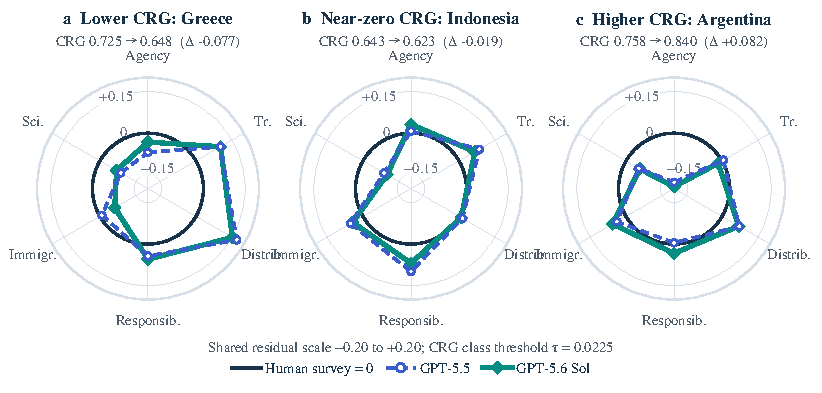
\includegraphics[width=\linewidth]{figs/figS5_country_profiles.pdf}
  \caption{Country-specific signed profiles spanning the CRG-change classes.
  \textbf{a}, Greece is the lower-CRG class medoid. \textbf{b}, Indonesia is the
  near-zero class medoid. \textbf{c}, Argentina is the higher-CRG class medoid.
  Every spoke is the model directed score minus that country's human-survey score;
  the black ring is zero and all panels share the $-0.20$ to $+0.20$ scale. Class
  medoids are descriptive views of heterogeneity; the full 64-country sample, rather
  than these cases, determines the estimates and uncertainty intervals.}
  \label{fig:country-profiles-appendix}
\end{figure}
\FloatBarrier
